\begin{figure*}[!t]
\centering
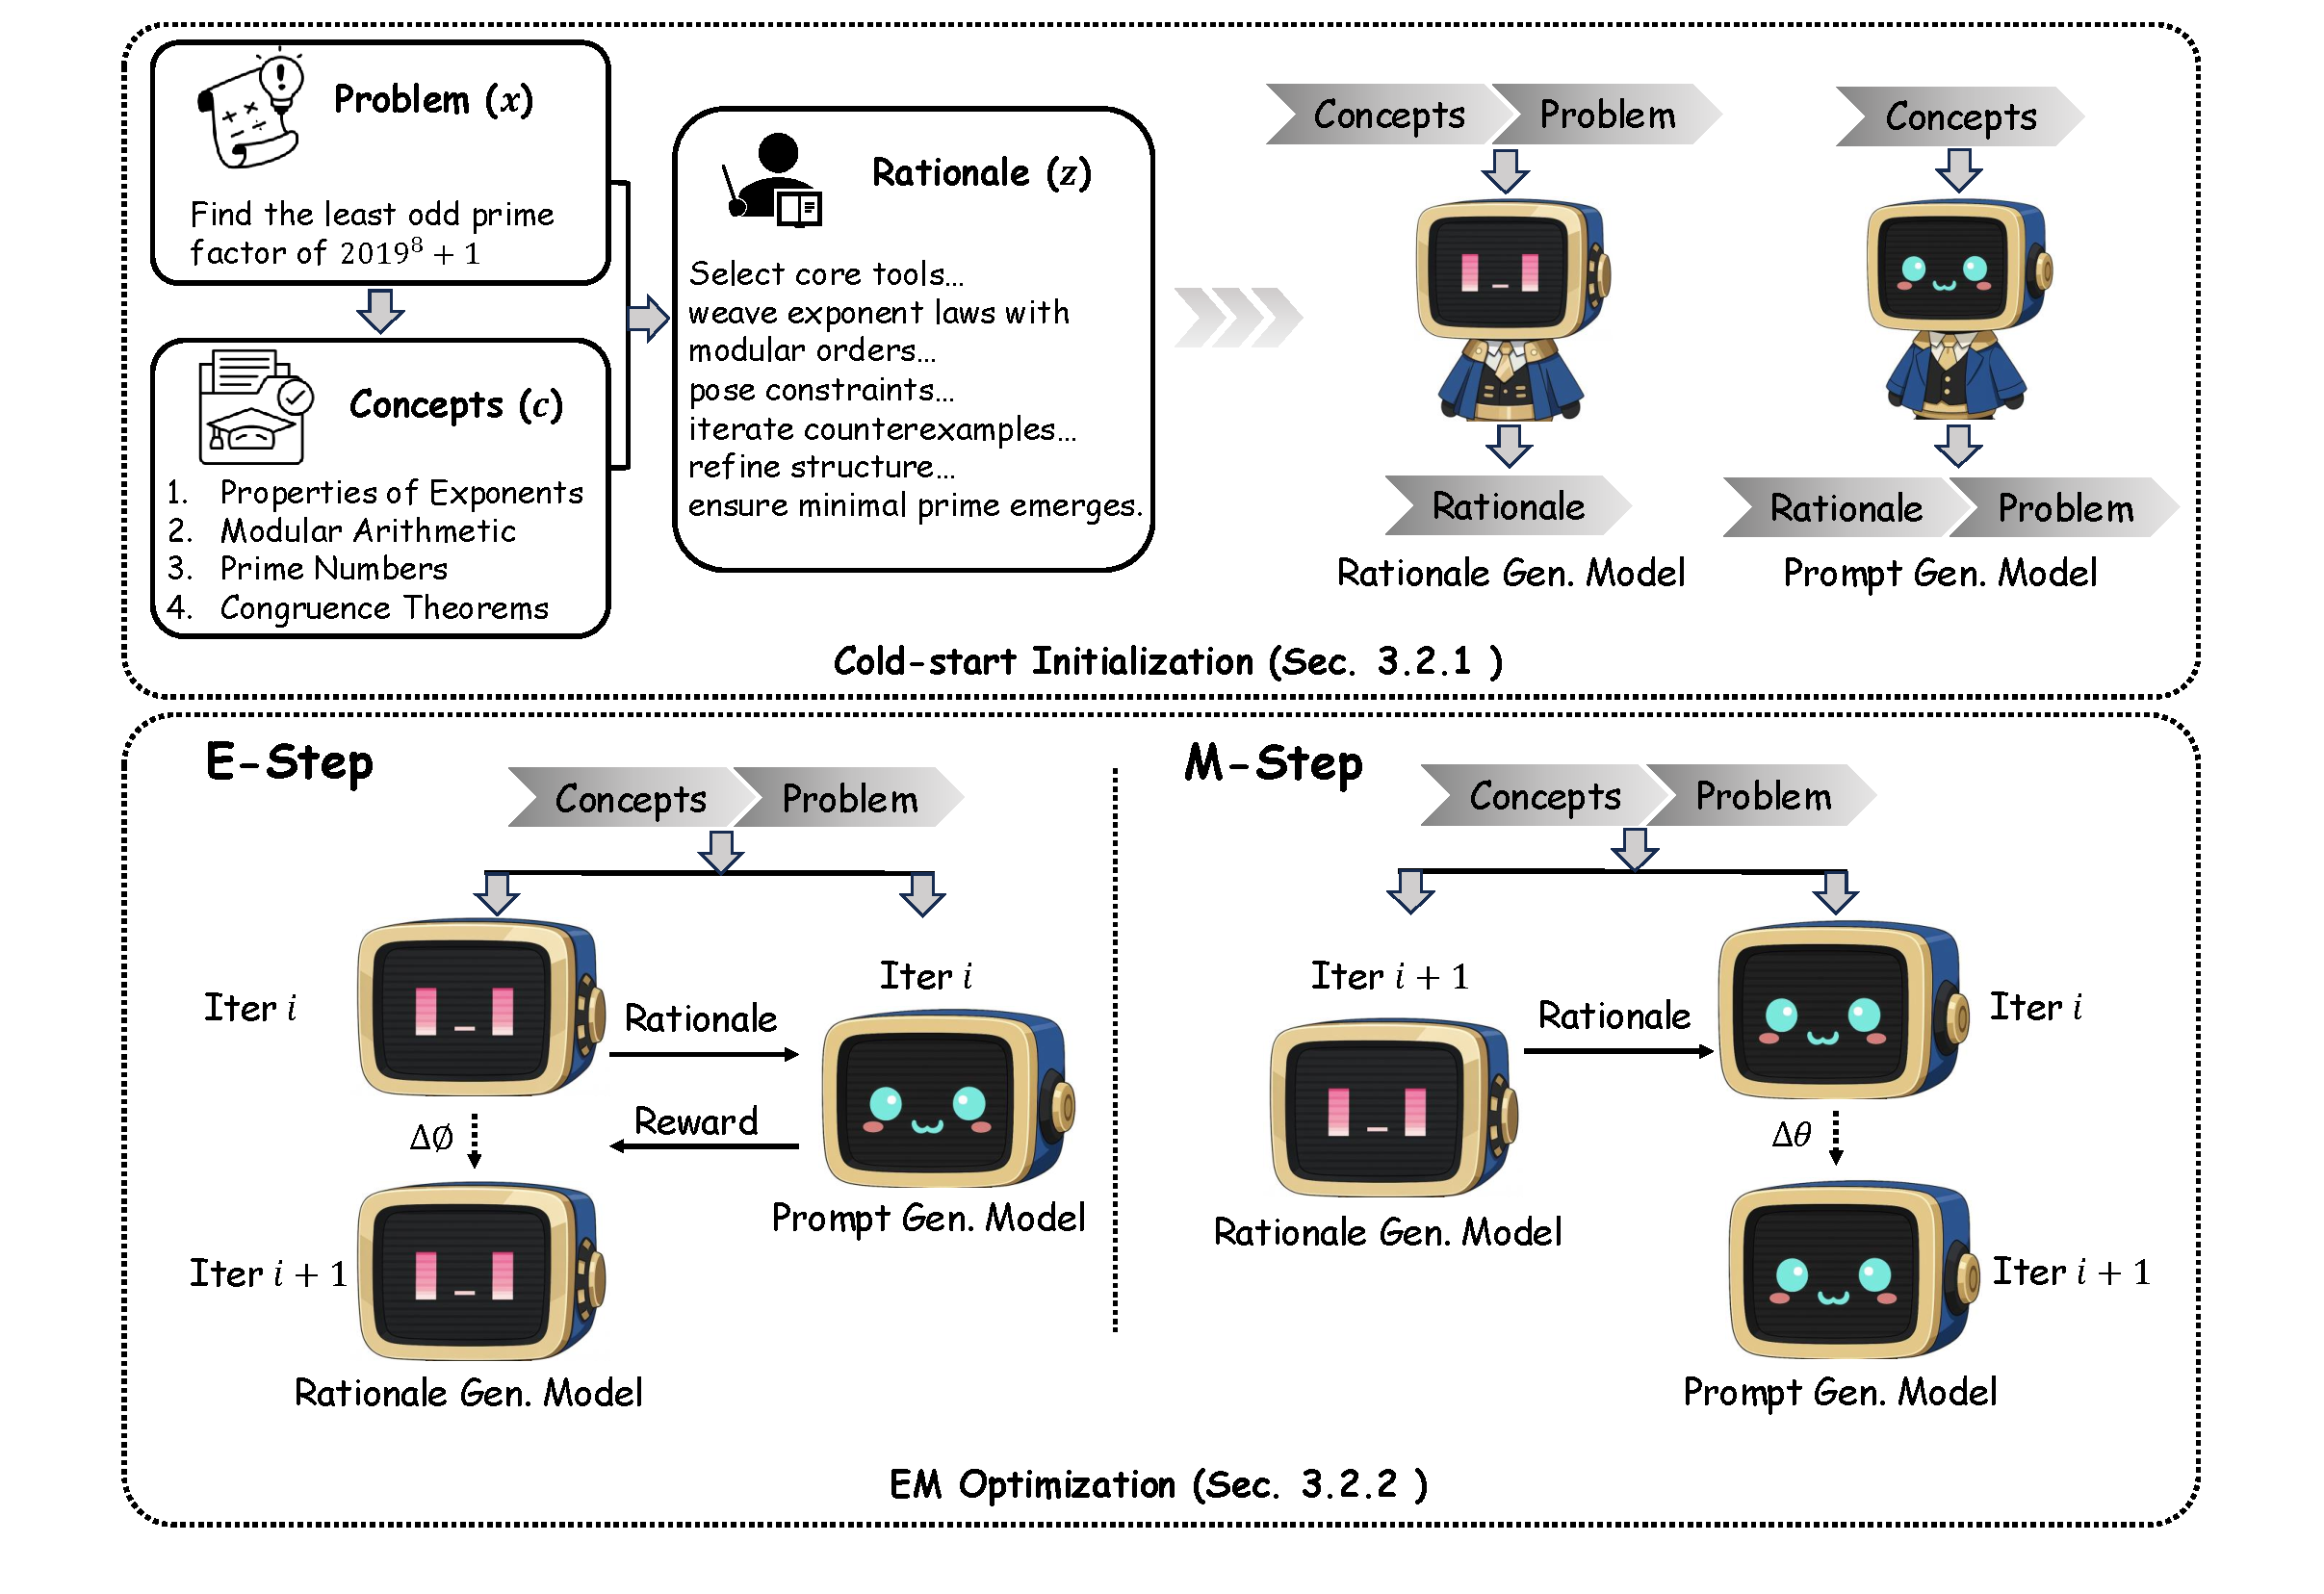
\includegraphics[width=0.8\textwidth]{promptcot2.pdf}
 % \vspace{-2mm}
\caption{Overview of PromptCoT 2.0.  
We begin with open-source problems and annotate their associated concepts and rationales, forming concept–rationale–problem triples that provide cold-start data for the rationale generation model and the prompt generation model.  
During EM optimization, the \textbf{E-step} updates the rationale generation model by maximizing the reward defined in Eq.~\ref{eq:reward}, while the \textbf{M-step} updates the prompt generation model to better align with the generated rationales.} 
\label{fig:method_overview} 
 % \vspace{-6mm}
 \end{figure*}


\section{Preliminaries}

\subsection{Problem Formulation: Prompt Synthesis}

We consider the setting where a prompt is constructed from a set of underlying concepts. Let $\mathcal{C}$ denote the concept space and $\mathcal{X}$ the prompt space. Each prompt $x \in \mathcal{X}$ is associated with a subset of concepts $\mathbf{c} \subseteq \mathcal{C}$. Prompt synthesis is then formulated as modeling the conditional distribution $p(x \mid \mathbf{c})$, with the objective of generating a prompt instance $x$ that faithfully reflects the specified concepts and ultimately enhances the reasoning capabilities of LLMs.

\subsection{The PromptCoT Framework}

A central challenge in prompt synthesis is that mapping concepts directly to prompts often yields underspecified or brittle problem statements~\citep{zhao2025promptcot}. To address this, PromptCoT~\citep{zhao2025promptcot} introduces an intermediate latent variable—the rationale. 
Instead of modeling $p(x \mid \mathbf{c})$ directly, PromptCoT factorizes it via rationales $z$, yielding:

\begin{equation}
\label{eq:marginal_likelihood}
p(x \mid \mathbf{c}) = \sum_{z} p(x \mid z, \mathbf{c})\, p(z \mid \mathbf{c}).
\end{equation}


The novelty of PromptCoT lies in its reframing of prompt synthesis: instead of constructing prompts directly from concepts, the process is mediated through rationales, such that prompts are derived jointly from the concepts and their explanatory structures. Rationales act as ``thinking process'' that grounds the concepts, decomposes them into intermediate explanatory steps, and guides the construction of more robust prompts. This shift has proven particularly effective in the mathematical domain~\citep{zhao2025promptcot}, where incorporating rationales substantially increases the difficulty of synthesized prompts and, in turn, yields significant improvements on challenging mathematical reasoning tasks.

While PromptCoT pioneers the exploration of the ``thinking mode'' in prompt synthesis, its reliance on human-crafted instructions and validation within a single domain highlight important limitations. The promising yet constrained empirical results, together with the technical limitations, motivate further investigation toward a more principled approach capable of enhancing the reasoning abilities of LLMs across broader tasks.


\section{PromptCoT~2.0}
We introduce PromptCoT~2.0 as a substantial advancement of the PromptCoT framework\footnote{To differentiate from the method introduced in this work, we denote the approach of \citep{zhao2025promptcot} as PromptCoT~1.0.}. An overview of the method is provided in Figure~\ref{fig:method_overview}, where a rationale generation model $q_\phi(z \mid \mathbf{c}, x)$ and a prompt generation model $p_\theta(z, x \mid \mathbf{c})$ are jointly trained under an Expectation–Maximization (EM) procedure.

In the E-step, $q_\phi(z \mid \mathbf{c}, x)$ is updated to assign higher probability to rationales that better connect concepts and prompts; while in the M-step, $p_\theta(z, x \mid \mathbf{c})$ is trained on concept–rationale–prompt triples $(\mathbf{c}, z, x)$, where rationales are inferred by the latest $q_\phi(z \mid \mathbf{c}, x)$. The objective is to maximize $\mathbb{E}_{q_\phi(z \mid \mathbf{c}, x)}[\log p_\theta(z, x \mid \mathbf{c})]$ over observed $(\mathbf{c}, x)$. Alternating these two steps progressively improves both $q_\phi(z \mid \mathbf{c}, x)$ and $p_\theta(z, x \mid \mathbf{c})$, creating an iterative loop in which rationales guide prompt construction and prompt synthesis, in turn, informs the discovery of more effective rationales.






\subsection{Variational Perspective}
\label{sec:variational}

Direct optimization of the marginal likelihood (Eq.~\ref{eq:marginal_likelihood}) is infeasible due to the summation over rationales. To address this, we introduce the approximate posterior $q_\phi(z \mid \mathbf{c}, x)$, yielding the evidence lower bound (ELBO):
\begin{equation}
\label{eq:elbo}
\log p_\theta(x \mid \mathbf{c}) \;\;\geq\;\; 
\mathbb{E}_{q_\phi(z \mid \mathbf{c}, x)} \big[\log p_\theta(z, x \mid \mathbf{c})\big] 
- \mathrm{KL}\!\left(q_\phi(z \mid \mathbf{c}, x)\,\|\,p_\theta(z \mid \mathbf{c})\right).
\end{equation}

This decomposition aligns naturally with the EM interpretation. In the E-step, maximizing the ELBO with respect to $q_\phi$ is equivalent to minimizing its KL divergence to the true posterior, whose optimal form is
\begin{equation}
\label{eq:posterior}
q_\phi^\star(z \mid \mathbf{c}, x) \;\propto\; p_\theta(z, x \mid \mathbf{c}) \;=\; p_\theta(x \mid z, \mathbf{c})\,p_\theta(z \mid \mathbf{c}).
\end{equation}
Thus, rationales are rewarded in proportion to their joint likelihood: they must align with the concepts while also being predictive of valid prompts.


In the M-step, with $q_\phi$ fixed, maximizing the ELBO reduces to maximizing the expected joint log-likelihood under the current posterior:
\begin{equation}
\label{eq:mstep}
\mathbb{E}_{q_\phi(z \mid \mathbf{c}, x)}\big[\log p_\theta(z, x \mid \mathbf{c})\big].
\end{equation}
This expectation provides the training signal for the prompt generation model: given observed pairs $(\mathbf{c}, x)$, rationales are sampled from $q_\phi(z \mid \mathbf{c}, x)$, and the model is updated to maximize the likelihood of reproducing the corresponding rationale–prompt pairs.

These updates establish a principled optimization loop: rationale generation is refined by rewards derived from prompt generation, and prompt generation is updated using rationales proposed by the posterior. The tight correspondence between the ELBO, the reward design, and the EM procedure ensures that both components improve in tandem, with rationales functioning as latent bridges between concepts and prompts.





\subsection{Practical Implementation}
\label{sec:implementation}
PromptCoT~2.0 is implemented as a two-phase training procedure, consisting of a cold-start initialization phase (\S\ref{sec:cold-start}) followed by an iterative EM optimization phase (\S\ref{sec:em}).



\subsubsection{Cold-start Initialization}
\label{sec:cold-start}

To bootstrap both the rationale generation model $q_\phi$ and the prompt generation model $p_\theta$, we follow the data construction procedure introduced in PromptCoT~1.0~\citep{zhao2025promptcot}. Specifically, we begin from open-source problem sets in mathematics and programming, and construct associated concept and rationale annotations. For each concept–problem pair $(\mathbf{c}, x)$, annotations are generated by prompting four high-capacity instruction-tuned models: \texttt{Qwen2.5-32B-Instruct}, \texttt{Qwen2.5-72B-Instruct}, \texttt{Llama-3.1-70B-Instruct} and \texttt{phi-4}. This procedure yields a seed corpus of concept–rationale–problem triples, which is then used to warm-start $q_\phi$ and $p_\theta$ via maximum likelihood estimation.



\subsubsection{EM Optimization}
\label{sec:em}

With the initial models in place, we proceed to optimize them jointly through the EM loop. In the E-step, the rationale generation model $q_\phi(z \mid \mathbf{c}, x)$ is updated via reinforcement learning, with the reward defined as
\begin{equation}
\label{eq:reward}
R(\mathbf{c}, x, z) = \log p_\theta(x \mid z, \mathbf{c}) + \log p_\theta(z \mid \mathbf{c}),
\end{equation}
which corresponds to the joint log-likelihood $\log p_\theta(z, x \mid \mathbf{c})$. 
Given a concept–prompt pair $(\mathbf{c}, x)$, rationales are sampled from $q_\phi(z \mid \mathbf{c}, x)$.  
For each pair, we draw eight candidate rationales and select the one with the highest reward; the parameters $\phi$ are then updated via supervised fine-tuning on this chosen rationale, ensuring that the model learns to prefer rationales that are both faithful to the concepts and predictive of valid prompts. 
In the M-step, the prompt generation model $p_\theta(z, x \mid \mathbf{c})$ is trained using the objective described in Eq.~\ref{eq:mstep}, leveraging rationales sampled from the current posterior. The two models are alternately updated until convergence, ensuring that $q_\phi$ aligns with the posterior distribution over rationales while $p_\theta$ adapts to rationales discovered in each iteration.





\section{LLM Post-Training with Synthesized Prompts}
\label{sec:downstream}
Armed with $p_\theta(z, x \mid \mathbf{c})$, we can construct a synthesized prompt dataset and post-train an LLM to enhance its reasoning capabilities. In PromptCoT~1.0, post-training is carried out through SFT, where reasoning traces and answers are distilled from strong teacher models. PromptCoT~2.0, by contrast, underscores the inherent limitations of SFT: as reasoning capabilities continue to advance, state-of-the-art LLMs demand ever-stronger teachers—models that are often inaccessible for distillation (e.g., proprietary models) or prohibitively expensive to employ (e.g., due to their massive parameter scale). To overcome these barriers, PromptCoT~2.0 moves beyond SFT and establishes a more broadly applicable post-training strategy, with a self-play regime at its core—enabling models to improve autonomously without dependence on increasingly powerful external teachers.



\paragraph{Self-Play.}  
For models that already possess strong reasoning capabilities (e.g., \texttt{Qwen3-30B-A3B-Thinking-2507}), the primary bottleneck shifts from the quality of supervision to the absence of even stronger teacher models for distillation. PromptCoT~2.0 overcomes this limitation by employing a self-play regime, where learning is guided by automatically verifiable feedback rather than relying on external traces.




Formally, given a collection of prompts $\{x_i\}_{i=1}^N$ with automatically verifiable signals~\footnote{This process requires no additional human annotation, as detailed in \S\ref{sec:details_post_train}.}, a base LLM $\mathcal{M}_\psi$ generates candidate solutions:
\[
y_i^{(j)} \;\sim\; \mathcal{M}_\psi(\cdot \mid x_i), \quad j=1,\dots,k.
\]
Each candidate is then assigned a scalar reward $u(x_i, y_i^{(j)}) \in \mathbb{R}$ derived from the corresponding verification signal. 
The general self-play objective is to update parameters $\psi$ to maximize expected reward:  
\[
\max_{\psi} \; \frac{1}{N} \sum_{i=1}^N \; \mathbb{E}_{y \sim \mathcal{M}_\psi(\cdot \mid x_i)} \big[ u(x_i, y) \big].
\]  

This framework is compatible with multiple optimization strategies, including PPO~\citep{schulman2017proximal}, GRPO~\citep{shao2024deepseekmath}, and DPO~\citep{rafailov2023direct}.
In all cases, the core mechanism is the same: the model improves by iteratively generating solutions, receiving feedback, and updating itself, without dependence on external teachers or human annotations.



\paragraph{Supervised Fine-Tuning.} For models that are not yet proficient in complex reasoning (e.g., \texttt{Qwen2.5-7B-Instruct}), self-play is no longer applicable. Instead, we employ a strong teacher model to generate complete reasoning traces for the synthesized prompts. The student model is then trained in a supervised manner on these problem–trace pairs, thereby acquiring reasoning behaviors directly from teacher demonstrations. This ensures that even weaker models can benefit effectively from PromptCoT~2.0 through explicit trajectory-level supervision.


